
\subsection{Mean Square Error, $R^2$ score, and optimal polynomial degree}

\autoref{fig:results_mse_values} shows us the MSE values and $R^2$ scores for our chosen range of  polynomial degrees. For the training data, we find from the MSE values that the optimal polynomial degree is $14$, while for the test data we find a polynomial degree $7$. This difference is expected, as for the training MSE values we train our model on a certain set of noise values, and the higher the polynomial the better the fit for that specific noise data set. However, when we then use the trained model to fit for the test data with new noise data points, the model is fitted so closely with the noise data points for the training data, that the model may no longer be a good fit for the test data. This is what we call \textit{overfitting}, and shows us that the highest polynomial degree is not necessarily the best one.

$R^2$ is the dimentionless \textit{coefficient of determination}, and it compares the model against the best constant 
prediction \cite{noauthor_machinelearninguiodocbookmllecturebookpdf_nodate}. The closer to $1$ the better the fit, and the closer to $0$, the worse the model. 

\begin{figure}[h!]
    \centering
    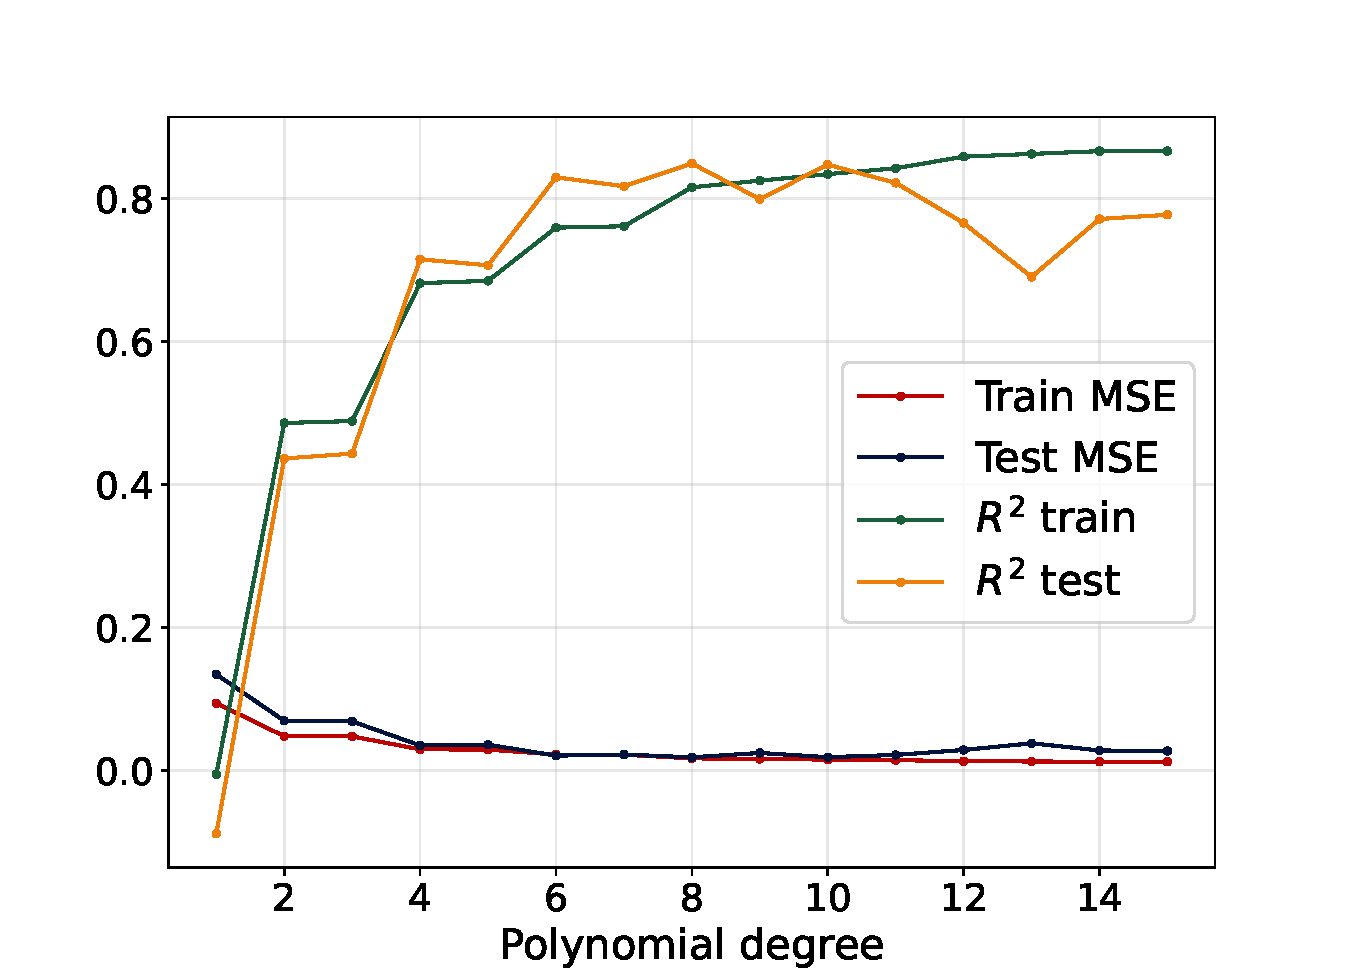
\includegraphics[width = 1.0\linewidth]{../figures/mse_values.pdf}
    \caption{Caption}
    \label{fig:results_mse_values}
\end{figure}